\section{问题一：单点往返运输能力与货箱组批}

\subsection{问题分析}

问题一不考虑实体无人机数量及共享电池周转，每个架次均采用
$O01\rightarrow S_i\rightarrow O01$ 的直接往返形式，且一个架次只能服务一个服务区。
因此，该问题可分为两个相互衔接的子问题：首先利用地形、航程和能量约束反解三种机型到各服务区的最大安全载荷；随后将同一服务区内不可拆分的货箱划分为若干批次，并联合选择机型，使架次数、运输能耗和累计作业时间尽可能小。

附件中的80个货箱只有4种质量--体积组合。利用这一离散结构，可以按箱型计数而非逐箱枚举，从而在较小状态空间内进行精确动态规划。考虑到灾后早期的组织负担和飞行风险，本文采用字典序多目标：首先最小化架次数，在此基础上最小化总能耗，最后最小化累计作业时间。

\subsection{航段几何、时间与能耗模型}

设机型集合为 $G=\{A,B,C\}$，服务区集合为 $S=\{S_1,\ldots,S_{15}\}$。
对任意节点 $i,j$，以两节点经纬度之间的测地距离作为水平巡航距离 $d_{ij}$。沿直线航段查询30~m DEM，记经过像元的最高高程为 $H_{ij}^{\max}$，则计划巡航海拔为
\begin{equation}
H_{ij}^{\mathrm{cruise}}=H_{ij}^{\max}+50.
\end{equation}
调度中心作业海拔取附件给定地面海拔，服务区作业海拔取地面海拔加30~m。由此得到航段爬升高度 $h_{ij}^{+}$ 和下降高度 $h_{ij}^{-}$。

机型 $g$ 携带载荷 $q$ 时的等效航程严格按题面给出的 $3/2$ 次幂关系计算。旋翼动量理论中的诱导功率随推力呈 $3/2$ 次幂变化，相关无人机配送能耗模型也讨论了载荷与能耗的联系；本文仍以题面公式为计算口径，不直接移用文献参数或数值结论\cite{zhang2021}：
\begin{equation}
L_g(q)=L_{g0}-\left(L_{g0}-L_{gF}\right)
\left(\frac{q}{Q_g}\right)^{3/2},\qquad 0\le q\le Q_g,
\end{equation}
其中，$L_{g0}$、$L_{gF}$ 和 $Q_g$ 分别为空载标准航程、满载标准航程和最大载货质量。
将单组电池可用能量 $E_g^{\mathrm{use}}$ 除以等效航程，得到单位水平距离能耗。航段总能耗为
\begin{equation}
E_{g,ij}(q)=\frac{E_g^{\mathrm{use}}}{L_g(q)}d_{ij}
+\frac{(m_g+q)g_0h_{ij}^{+}}{3.6\times10^6\eta_g},
\end{equation}
其中 $m_g$ 为空机质量，$g_0=9.80665~\mathrm{m/s^2}$，$\eta_g$ 为爬升能耗效率。按照题面规定，下降过程不单独计算附加能耗。

单点投送后货物已全部卸载，故返程有效载荷为0。载质量为 $q$ 的往返架次能耗为
\begin{equation}
E_{g,i}^{\mathrm{rt}}(q)=E_{g,O01,i}(q)+E_{g,i,O01}(0).
\end{equation}
若本架次装载 $n$ 个货箱，其完整作业时间为
\begin{equation}
T_{g,i}(n)=T_g^{\mathrm{prep}}+T_g^{\mathrm{load}}n
+\sum_{(u,v)\in\{(O01,i),(i,O01)\}}
\left(\frac{h_{uv}^{+}}{v_g^{\uparrow}}+\frac{d_{uv}}{v_g^c}+\frac{h_{uv}^{-}}{v_g^{\downarrow}}\right)
+T_g^{\mathrm{handoff}}+T_g^{\mathrm{perbox}}n.
\end{equation}
该式同时计入固定准备、逐箱装载、往返飞行、基础交接和逐箱交接时间。由于问题一明确不考虑实体无人机调度，本文将所有架次完整作业时间之和作为“累计作业时间”，不将其解释为多机并行条件下的完工时间。

\subsection{最大安全载荷反解}

设机型 $g$ 的返航安全余量为 $\rho_g$。最大安全载荷 $q_{g,i}^{\max}$ 满足
\begin{equation}
q_{g,i}^{\max}=\max\left\{q:\ 0\le q\le Q_g,
\ E_{g,i}^{\mathrm{rt}}(q)\le(1-\rho_g)E_g^{\mathrm{use}}\right\}.
\end{equation}
由于 $L_g(q)$ 随载荷单调减小，往返能耗随载荷单调增加，故采用二分法求解该一维边界。取附件默认安全余量 $\rho_g=20\%$，结果见表~\ref{tab:q1-payload}。

\begin{table}[htbp]
\centering
\caption{20\%返航安全余量下各机型最大安全载荷（kg）}
\label{tab:q1-payload}
\small
\begin{tabular}{cccccccc}
\toprule
服务区 & A型 & B型 & C型 & 服务区 & A型 & B型 & C型\\
\midrule
S001 & 25.000 & 30.000 & 80.000 & S009 & 25.000 & 30.000 & 80.000\\
S002 & 25.000 & 30.000 & 68.554 & S010 & 25.000 & 30.000 & 80.000\\
S003 & 25.000 & 30.000 & 68.235 & S011 & 25.000 & 30.000 & 80.000\\
S004 & 25.000 & 30.000 & 63.259 & S012 & 25.000 & 30.000 & 68.015\\
S005 & 25.000 & 30.000 & 80.000 & S013 & 25.000 & 30.000 & 80.000\\
S006 & 25.000 & 30.000 & 80.000 & S014 & 25.000 & 30.000 & 80.000\\
S007 & 25.000 & 30.000 & 80.000 & S015 & 25.000 & 30.000 & 80.000\\
S008 & 25.000 & 28.632 & 58.436 & & & &\\
\bottomrule
\end{tabular}
\end{table}

结果表明，A型除受自身25~kg载荷上限约束外，在全部服务区均可满载；B型仅在S008受能量约束而不能满载；C型在S002、S003、S004、S008和S012受长航程或较大爬升高度影响，最大安全载荷低于80~kg。各服务区载荷边界及机型额定载荷对照见图~\ref{fig:q1-payload}。
\begin{figure}[htbp]
\centering
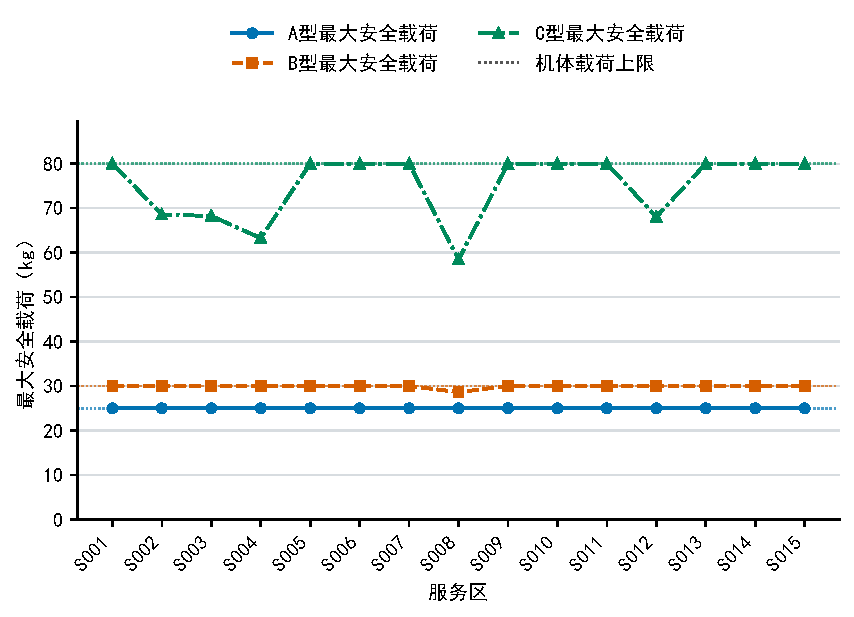
\includegraphics[width=0.96\textwidth]{figures/q1_payload_by_service.pdf}
\caption{20\%返航安全余量下各服务区的机型最大安全载荷}
\label{fig:q1-payload}
\end{figure}

\subsection{跨机型货箱组批模型}

将医疗物资、饮用水、应急食品和生活卫生用品依次记为4种箱型。对服务区 $i$，用向量 $\boldsymbol{b}_i$ 表示各箱型需求数量。枚举机型 $g$ 下所有满足质量、体积和能量限制的装载组合，构成可行选项集合 $\mathcal{F}_i$。对选项 $r\in\mathcal{F}_i$，记其箱型计数向量为 $\boldsymbol{a}_r$，能耗和作业时间分别为 $e_r,t_r$，决策变量 $x_r$ 表示该选项使用的架次数。模型为
\begin{align}
\operatorname{lexmin}\quad &
\left(\sum_{r\in\mathcal{F}_i}x_r,
\sum_{r\in\mathcal{F}_i}e_rx_r,
\sum_{r\in\mathcal{F}_i}t_rx_r\right),\\
\text{s.t.}\quad &
\sum_{r\in\mathcal{F}_i}\boldsymbol{a}_rx_r=\boldsymbol{b}_i,\\
&x_r\in\mathbb{Z}_{\ge0}.
\end{align}
等式约束保证每个货箱恰好分配一次；可行选项的生成过程已经内嵌载质量、装载体积和返航安全余量约束。

求解时以“尚未分配的4类货箱数量”为动态规划状态。对每个状态枚举一个可行架次，转移到扣除对应货箱后的新状态，并依次比较架次数、累计能耗和累计时间。全题单服务区最大状态数为 $(2+1)(8+1)(3+1)(2+1)=324$，三种机型对应的候选装载上界不足 $3\times323=969$，可对全部状态和选项进行穷尽搜索。所得解是上述字典序目标下的精确最优解，不依赖随机初值，也不存在启发式算法的收敛误差。

\subsection{组批结果与多目标权衡}

各服务区联合最优结果见表~\ref{tab:q1-plan-summary}，逐箱货箱编号及每架次质量、体积、能耗、时间和返航SOC见结果附件。

\begin{table}[htbp]
\centering
\caption{各服务区联合最优组批结果}
\label{tab:q1-plan-summary}
\small
\begin{tabular}{ccrrr}
\toprule
服务区 & 机型组合 & 架次数 & 能耗/kWh & 时间/s\\
\midrule
S001 & C+C & 2 & 5.9309 & 3188.9\\
S002 & C+B & 2 & 8.4612 & 3864.9\\
S003 & C+B & 2 & 8.5424 & 4450.1\\
S004 & C & 1 & 6.1769 & 2305.2\\
S005 & C & 1 & 4.2387 & 1880.0\\
S006 & C & 1 & 2.5939 & 1560.9\\
S007 & C & 1 & 3.4104 & 1907.5\\
S008 & C & 1 & 5.8575 & 2203.8\\
S009 & B & 1 & 2.1024 & 1560.8\\
S010 & B & 1 & 1.8210 & 1554.6\\
S011 & B & 1 & 1.0771 & 1189.6\\
S012 & B & 1 & 2.7552 & 1923.8\\
S013 & B & 1 & 1.8245 & 1510.4\\
S014 & B & 1 & 2.1372 & 1868.6\\
S015 & B & 1 & 2.3108 & 1829.6\\
\midrule
合计 & B型9+C型9 & 18 & 59.2403 & 32798.5\\
\bottomrule
\end{tabular}
\end{table}

18架次不仅是算法得到的结果，也可由下界证明。每个服务区至少需要1架次；S001、S002和S003的需求总质量分别为154、81和81~kg，均超过单架最大载荷80~kg，故三者各至少需要2架次。因此总架次数下界为
\begin{equation}
15+3=18,
\end{equation}
本文方案达到该下界，故架次数全局最优。

为说明三个目标之间的权衡，分别限制全程只使用一种机型，并与跨机型联合方案比较，结果见表~\ref{tab:q1-tradeoff}。

\begin{table}[htbp]
\centering
\caption{不同机型策略的指标比较}
\label{tab:q1-tradeoff}
\begin{tabular}{lrrr}
\toprule
策略 & 架次数 & 总能耗/kWh & 累计作业时间/s\\
\midrule
仅A型 & 52 & 112.383 & 89415.8\\
仅B型 & 35 & 68.478 & 55708.7\\
仅C型 & 18 & 74.058 & 33861.2\\
跨机型联合优化 & 18 & 59.2403 & 32798.5\\
\bottomrule
\end{tabular}
\end{table}

仅使用C型已能达到最少架次数，但在小批量服务区存在“大机小载”现象。联合方案保持18架次不变，同时用B型承担S009--S015以及S002、S003中的小批量，使能耗较仅C型下降约20.0\%，累计作业时间下降约3.1\%。这说明“最少架次数”并不自动对应“最低能耗”，异构机型组合能够改善次级目标。

\subsection{安全余量灵敏度分析}

以附件默认值20\%为中心，为同时覆盖宽松情景与方案失效边界，将返航安全余量 $\rho$ 从0逐步提高到40\%，每个取值下重新生成可行装载组合并执行跨机型联合优化。

\begin{table}[htbp]
\centering
\caption{返航安全余量对全局组批方案的影响}
\label{tab:q1-sensitivity}
\small
\begin{tabular}{crrrccc}
\toprule
$\rho$ & 架次数 & 总能耗/kWh & 时间/s & A型 & B型 & C型\\
\midrule
0\%--20\% & 18 & 59.2403 & 32798.5 & 0 & 9 & 9\\
25\% & 19 & 61.1897 & 34592.3 & 0 & 10 & 9\\
30\% & 20 & 67.3577 & 36616.8 & 0 & 9 & 11\\
35\% & 25 & 78.1856 & 45550.8 & 0 & 14 & 11\\
40\% & \multicolumn{6}{c}{不可行}\\
\bottomrule
\end{tabular}
\end{table}

在0--20\%范围内，18架次方案及机型结构保持不变，说明默认20\%余量下结论稳定。当余量升至25\%时，部分长航程服务区的单架安全载荷跨过组批临界值，架次数增至19；30\%和35\%时进一步增至20和25。余量达到40\%后，S004、S008等长航程服务区出现至少一种较重货箱无法由任何机型安全运输的情况，问题转为不可行。因此，20\%是兼顾安全性与运输效率的稳定取值，而25\%是当前方案架次数发生变化的首个临界点。全局架次、能耗和累计作业时间的变化趋势见图~\ref{fig:q1-sensitivity}；40\%处因不存在可行装载组合而停止绘制指标值。
\begin{figure}[htbp]
\centering
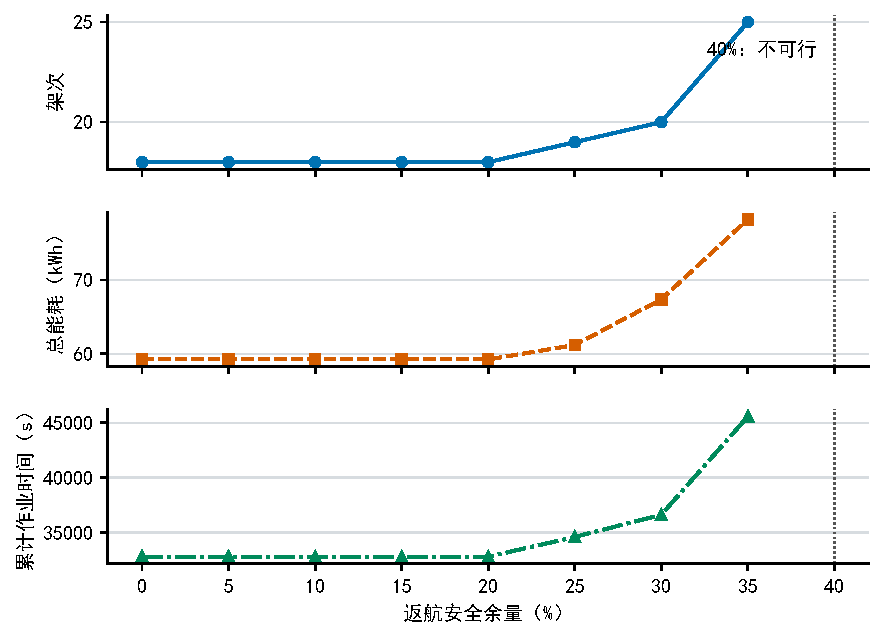
\includegraphics[width=0.96\textwidth]{figures/q1_global_reserve_sensitivity.pdf}
\caption{返航安全余量对全局组批方案指标的影响}
\label{fig:q1-sensitivity}
\end{figure}

\subsection{模型检验与误差讨论}

本文从以下方面进行独立复核：其一，检查 $L_g(0)=L_{g0}$、$L_g(Q_g)=L_{gF}$ 以及载荷增加时能耗单调增加；其二，重新读取逐箱结果，验证80个货箱恰好出现一次，总质量758.0~kg、总体积2.011~m$^3$，并逐架次复算质量、体积、能量、时间和SOC；其三，以18架次解析下界验证动态规划的最优性。上述检查均通过。程序在Python~3.13环境下运行，主要使用NumPy~2.2.5、SciPy~1.15.3和openpyxl~3.1.5；求解入口与独立检查入口分别为 \texttt{q1\_sensitivity.py} 和 \texttt{q1\_validate.py}。

误差主要来自三个方面：DEM为空间分辨率约30~m的栅格数据，航段最高高程受像元采样影响；附件节点海拔与DEM采样值存在不超过10.6~m的偏差，本文按题意以附件海拔作为作业高度、DEM仅用于沿线净空；等效航程模型把实际复杂飞行过程折算为确定性单位距离能耗，未显式考虑风速和电池老化。为评估空间离散误差，将沿线采样密度由每像元跨度约1点提高到8点，个别航段最高高程最多增加10.14~m，总能耗由59.2232增至59.2403~kWh（约0.03\%），累计时间由32755.1增至32798.5~s（约0.13\%），18架次及B型9架次、C型9架次的结构保持不变。由于题目未提供风场与电池老化数据，这些因素不纳入主模型，其影响通过返航安全余量吸收。安全余量灵敏度结果表明，在0--20\%范围内最优架次数和机型结构均不变，故上述误差不足以改变问题一的核心结论。
